\documentclass[12pt]{article}

\usepackage{amsmath}
\usepackage{amssymb}
\DeclareMathOperator*{\argmin}{arg\,min}

\usepackage{graphicx}
\graphicspath{ {paper_figures/} }

\usepackage{forloop}

\begin{document}

\section{Introduction}

% only images

\section{Techniques}

% show schematic with images (starfish or zebrafish w/ stripes)

\subsection{Alignment Using Angular Synchronization}

Often when we collect images in experiments, each image is taken in a different orientation. 
%
Therefore, the first task in image analysis is to align the set of images. 
%
We will consider settings when alignment is done with respect to two--dimensional translations and rotations of the images, as each ``object of interest'' (i.e. each embryo) is in a different position and rotated at a different angle within the image frame. 

There are many ways to align images. 
%
``Template--based'' alignment \cite{ahuja2007template} is one technique, where one selects a specific image or {\em template}, and then tries to optimally align each image to that template.
%
However, this method can result in many misalignemnts for noisy images, and can be problematic if a ``good'' template image is not known {\em a priori}. 
%
Instead, we will use a technique called angular synchronization\cite{singer2011angular} to align our sets of images.
%
Angular synchronization first computes the pairwise alignments for every possible pair of images, effectively using each image as a template for every other image.
%
From this large collection of pairwise alignments, it then tries to find optimal alignment for each image, such that these individual alignments are most consistent (in some metric) with the pairwise alignment.
%
Because we consider {\em all} pairwise alignments, angular synchronization is often much more robust to noise. 

An important part of angular synchronization is that the symmetry group $G$ be {\em compact} and have a real (or perhaps complex) representation \cite{singer2011angular}.
%
Compactness guarantees (by the extreme value theorem) that the minimizer for each pairwise alignment is contained in the group,
and having a real representation allows us to write combinations of transforms as group operations, which will allow us to therefore write our optimization problem in matrix form. 
%
This is a rather technical point;
we are only discussing this because the group of two--dimensional translations and rotations, $ISO(2)$, is {\em not} compact.
%
The angular synchronization problem is therefore not well--defined for this symmetry group.
%
However, we can ``compactify'' this group by mapping $ISO(2)$ to the group $SO(3)$, the group of three--dimensional rotations.
%
We do this by projecting the image onto a portion of the surface of a (three--dimensional) sphere.
%
Rotations in two--dimensions now correspond to rotations around one principal axis in three--dimensions, and translations in two--dimensions correspond (approximately) to rotations around the other two principal axes in three--dimensions.
%
Furthermore, successive applications of various translations and rotations can be described via multiplication of the corresponding rotation matrices in $SO(3)$.

Let $x_1, \dots, x_m \in \mathbb{R}^{n \times n}$ denote the (grayscale) images that we wish to align with respect to translations and rotations.
%
The first step in angular synchronization is to compute the translations and rotations to optimally align each pair of data points. 
%
For each image pair $x_i$ and $x_j$, we would like to solve
\begin{equation}\label{eq:opt_pairwise}
(\theta_{ij}, dx_{ij}, dy_{ij}) = \argmin_{\theta \in [0, 2\pi), dx \in [-\Delta, \Delta], dy \in [-\Delta, \Delta]} \|f(x_j, \theta, dx, dy) - x_i \|_F^2.
\end{equation}
where $\| \cdot \|_F$ denotes the Frobenius norm, and $f$ is a function that first rotates the image $x_j$ by $\theta$ degrees, then translates the image by $dx$ pixels in the $x$ direction, and finally translates the image by $dy$ pixels in the $y$ direction. 
%
$\Delta$ is the maximum number of pixels by which we are allowed to translate the image; we take $\Delta=20$, which corresponds to a 20\% shift in the image, $\Delta$ can be taken larger or smaller depending on the nature of the images. 
%
The solution to \eqref{eq:opt_pairwise} is not easily computed, as the objective function will most likely be nonconvex.
%
Therefore, instead of using an optimization procedure to compute the solution to \eqref{eq:opt_pairwise}, we choose to discretize the search space and exhaustively search to estimate the solution to \eqref{eq:opt_pairwise}.
%
We discritize the search space of rotations into 20 possible rotations ($0, \pi/10, \pi/5, \dots, 9 \pi/5, 19\pi/10$), and 11 possible translations in both the $x$ and $y$ directions ($-20, -16, -12, \dots, 12, 16, 20$ pixels). 
%
We then check all possible combinations for the best rotation and translations that align $x_i$ to $x_j$. 
%
Although this can be somewhat time intensive, it is not prohibitive for the size of data sets which we are considering, and can be trivially parallelized for larger data sets if necessary.
%
The solution to this search will not be the exact solution to \eqref{eq:opt_pairwise}, but it will (most likely) be a close approximation.
%
Since our techniques are robust to noise, close approximations will be sufficient to obtain accurate results.

We now compute the three--dimensional rotation, $R_{ij} \in SO(3)$, from the two--dimensional parameters $\theta_{ij}$, $dx_{ij}$, and $dy_{ij}$.
%
In the space of three--dimensional rotations, the Euler angles $\alpha_{ij}$, $\beta_{ij}$, and $\gamma_{ij}$ correspond to
\begin{equation} \label{eq:angle_relations}
\begin{aligned}
	\alpha_{ij} &= \theta_{ij} \\
	\beta_{ij} &= \frac{dx_{ij}}{n} \times \eta_{proj} \\
	\gamma_{ij} &= \frac{dy_{ij}}{n} \times \eta_{proj} \\
\end{aligned}
\end{equation}
where $\eta_{proj}$ is the angular portion of the sphere onto which we choose to project (we take $\eta_{proj} =  \pi/8$).
%
From here, we can write rotations around the three principal axes in terms of the three Euler angles
\begin{equation}
\begin{aligned}
	R^x_{ij} &= \begin{bmatrix}
	1 & 0 & 0 \\
    0 & \cos(\alpha) & -\sin(\alpha) \\
    0 & \sin(\alpha) & \cos(\alpha)
	\end{bmatrix} \\
	R^y_{ij} &= \begin{bmatrix}
	\cos(\beta) & 0 & \sin(\beta) \\
    0 & 1 & 0 \\
    -\sin(\beta) & 0 & \cos(\beta)
    \end{bmatrix} \\
	R^z_{ij} &= \begin{bmatrix} 
	\cos(\gamma) & -\sin(\gamma) & 0 \\
    \sin(\gamma) & \cos(\gamma) & 0 \\
    0 & 0 & 1 
    \end{bmatrix}
\end{aligned}
\end{equation}
where $R^x_{ij}$, $R^y_{ij}$, and $R^z_{ij}$ correspond to rotations around the $x$, $y$, and $z$ axes, respectively.
%
We then write the total rotation $R_{ij} \in SO(3)$ as 
\begin{equation} \label{eq:total_rot}
	R_{ij}	 = R^z_{ij} \times R^y_{ij} \times R^x_{ij}
\end{equation}
%
This corresponds to first rotating the image by $\theta$, then translating the image by $dx$ pixels in the $x$ direction, and finally translating the image by $dy$ pixels in the $y$ direction (we note that, because the rotation matrices operate from the left, the rightmost rotation matrix in the product in \eqref{eq:total_rot} corresponds to the first operation we perform on the image).


Given the pairwise rotations that optimally align the imges, $R_{ij}$, we would like to find the rotations $R_1, R_2, \dots, R_n \in SO(3)$ such that $R_i R_j^T \approx R_{ij}$, for every pair $i, j$. 
%TODO: Check that this order is correct
%
We would also like to exploit {\em higher-order} consistency relations;
for example, the relationship $R_{ij} R_{jk} \approx R_{ik}$ should hold if the rotation estimates are accurate.
%
Therefore, we consider measurements which (almost) satisfy such conditions ``good'' measurements, and those measurements which do not satisfy such conditions as most likely inaccurate.


We formulate our problem as an optimization problem:
\begin{equation} \label{eqn:angsynch_obj}
\max_{R_1, \dots, R_m \in SO(3)} \left\| \sum_{i=1}^{m} \sum_{j=1}^{m} R_i^T R_{ij} R_j \right\|^2.
\end{equation}
%
%TODO: check if a norm is needed
Each term in the objective function will be large large if $R_i$ and $R_j$ are consistent with $R_{ij}$, and will be random with mean 0 if $R_i$ and $R_j$ are inconsistent with $R_{ij}$.
%
Therefore, solving \eqref{eqn:angsynch_obj} gives us the set of global alignments which are most consistent with the computed pairwise alignments.

In general, the solution to \eqref{eqn:angsynch_obj} is not easily computed.
%
Instead, we relax the problem and allow $R_1, \dots, R_m \in \mathbb{R}^{3 \times 3}$.
%
We define the matrix $H \in \mathbb{R}^{3m \times 3m}$, which is an $m \times m$ block matrix with $3 \times 3$ blocks, with $H_{ij} = R_{ij}$.
%
We can then write the relaxed problem as 
\begin{equation} \label{eqn:angsynch_relax}
\max_{R\in \mathbb{R}^{3m \times 3}} \| R^T H R \|^2.
\end{equation}
%
The solution to \eqref{eqn:angsynch_relax} is given by the top ``block'' eigenvector of $H$, which we denote $\hat{R} \in \mathbb{R}^{3m \times 3}$. 
%
The $i^{th}$ rotation is (approximately) the $i^{th}$ block of $\hat{R}$, $\hat{R}(i) \in \mathbb{R}^{3 \times 3}$.
%
We would like to note that this formulation also accounts for higher-order relations.
%
For example, if we want to optimize over all pairs of pairwise rotations, we would solve $\max_{R_1, \dots, R_m \in SO(3)} \sum_{i=1}^{m} \sum_{j=1}^{m} \left\| R_i^T \left( \sum_k R_{ik} R_{kj} \right) R_j \right\| = \| R^T H^2 R \|^2$. 
%
However, the solution to this problem is also given by the top eigenvector of $H$. 

Because we relaxed the problem to allow our solutions to lie in $\mathbb{R}^{3 \times 3}$, we must project our approximate solution back to $SO(3)$.
%
The optimal rotation is therefore given by $R_i = U_i V_i^T$, where $U_i$ and $V_i$ are the left and right singular vectors of $\hat{R}_i$, respectively \cite{...}. 
%
Because the eigenvectors of $H$ are determined up to a sign, we adjust the signs of the eigenvectors so that $det(R_i) = +1$ to ensure proper rotations.
%

From the matrices $R_1, \dots, R_m$, we now wish to find the corresponding translations and rotations of the images.
%
Because we are permitted to adjust our rotations by a global rotations, we multiply all rotations by $R_1^T$ to ensure that all the images are (approximately) in the same region of the sphere where we began.
%
We then compute the Euler angles $\alpha$, $\beta$, and $\gamma$ from the rotation matrix $R$ using the following relationships
\begin{equation}
\begin{aligned}
R_{1,1} & = \cos(\beta)\cos(\gamma) \\
R_{2,1} & = \cos(\beta)\sin(\gamma) \\
R_{3,1} & = -\sin(\beta) \\
R_{3,2} & = \sin(\alpha)\cos(\beta) \\
R_{3,3} & = \cos(\alpha)\cos(\beta) 
\end{aligned}
\end{equation}
%
We can then invert \eqref{eq:angle_relations} to compute the optimal translation and rotation for each image.

\subsection{Ordering Using Diffusion Maps}

Given our set of aligned images, we wish to order them {\em in time} so that we can reconstruct the developmental dynamics.
%
We will use diffusion maps (DMAPS) \cite{coifman2005geometric} to temporally order our data.
%
DMAPS aims to uncover a parameterization of high-dimensional data sampled from a low-dimensional nonlinear manifold.
%
The {\em essential} requirement for DMAPS is an appropriate distance metric $d(x_i, x_j)$ for comparing data points. 
%
This can as simple as the standard Euclidean distance, or a more complex metric (such as a distance between features of the data points) for other data sets.
%
We will use the Frobenius norm of the difference of our aligned pictures as our distance metric, $d(x_i, x_j) = \| x_i - x_j \|_F$.

Given {\em aligned} images $x_1, \dots, x_m \in \mathbb{R}^{n \times n}$, we fist calculate the matrix $W \in \mathbb{R}^{m \times m}$, where 
\begin{equation}
W_{ij} = \exp \left( -\frac{d^2(x_i, x_j)}{\epsilon^2} \right)
\end{equation}
and $\epsilon$ is a characteristic distance between data points.
%
$\epsilon$ can be chosen using several techniques (see, for example \cite{coifman2008graph}); in practice, we choose $\epsilon$ to be the median of the pairwise distances between data points.
%
We then compute the diagonal matrix $D$, where $D_{ii} = \sum_{j=1}^{m} W_{ij}$, and the matrix $A = D^{-1} W$. 
%
We calculate the eigenvectors $\phi_1, \phi_2, \dots, \phi_m$ and eigenvalues $\lambda_1, \lambda_2, \dots, \lambda_m$ and order them such that $|\lambda_1| \ge |\lambda_2| \ge \dots \ge |\lambda_m|$. 
%
Because the matrix $A$ is similar to the symmetric matrix $D^{-1/2} W D^{-1/2}$, $A$ is guaranteed to have real eigenvalues and real, orthogonal eigenvectors. 
%
The eigenvectors $\phi_1, \phi_2, \dots, \phi_m$ give the embedding coordinates, such that $\phi_j(i)$ gives the $j^{th}$ embedding coordinate of the $i^{th}$ data point. 
%
Because the matrix $A$ is row-stochastic, $\lambda_1=1$ and $\phi_1$ is a constant vector.
%
The next few eigenvectors give the ``meaningful'' embedding coordinates for the data. 

In our setup, we assume that our data are inherently one--dimensional, and that this one dimension is correlated with time.
%
Therefore, ordering our data by $\phi_2(j)$ will allow us to automatically order our data in time. 

\subsection{Vector Diffusion Maps}

Many times, we would to both align and order our data.
%
Our proposed alignment methodology, angular syncrhonization, utilizes the eigendecompostion of the matrix $R \in \mathbb{R}^{3m \times 3m}$, and our proposed ordering algorithm, diffusion maps, utilizes the eigendecomposition of the matrix $A \in \mathbb{R}^{m \times m}$.
%
We can combine the two steps into one eigencomputation that allows us to {|em simultaneously} recover the optimal alignments and the temporal ordering.
%
This technique is called vector diffusion maps \cite{singer2012vector}.
%
It is significantly more robust to mistakes in the alignment.

For vector diffusion maps, we construct the matrix $S \in \mathbb{R}^{3m \times 3m}$

\section{Example: {\em Drosophila}}

\subsection{dpERK}

\def \nimages {81}
\def \imagewidth {0.22in}
\begin{figure}
\begin{minipage}{0.5\textwidth}
\newcounter{n}
\forloop{n}{1}{\value{n} < \nimages}{
	\includegraphics[width=\imagewidth]{dpERK_\arabic{n}}
}
\hspace{0pt}
\end{minipage}
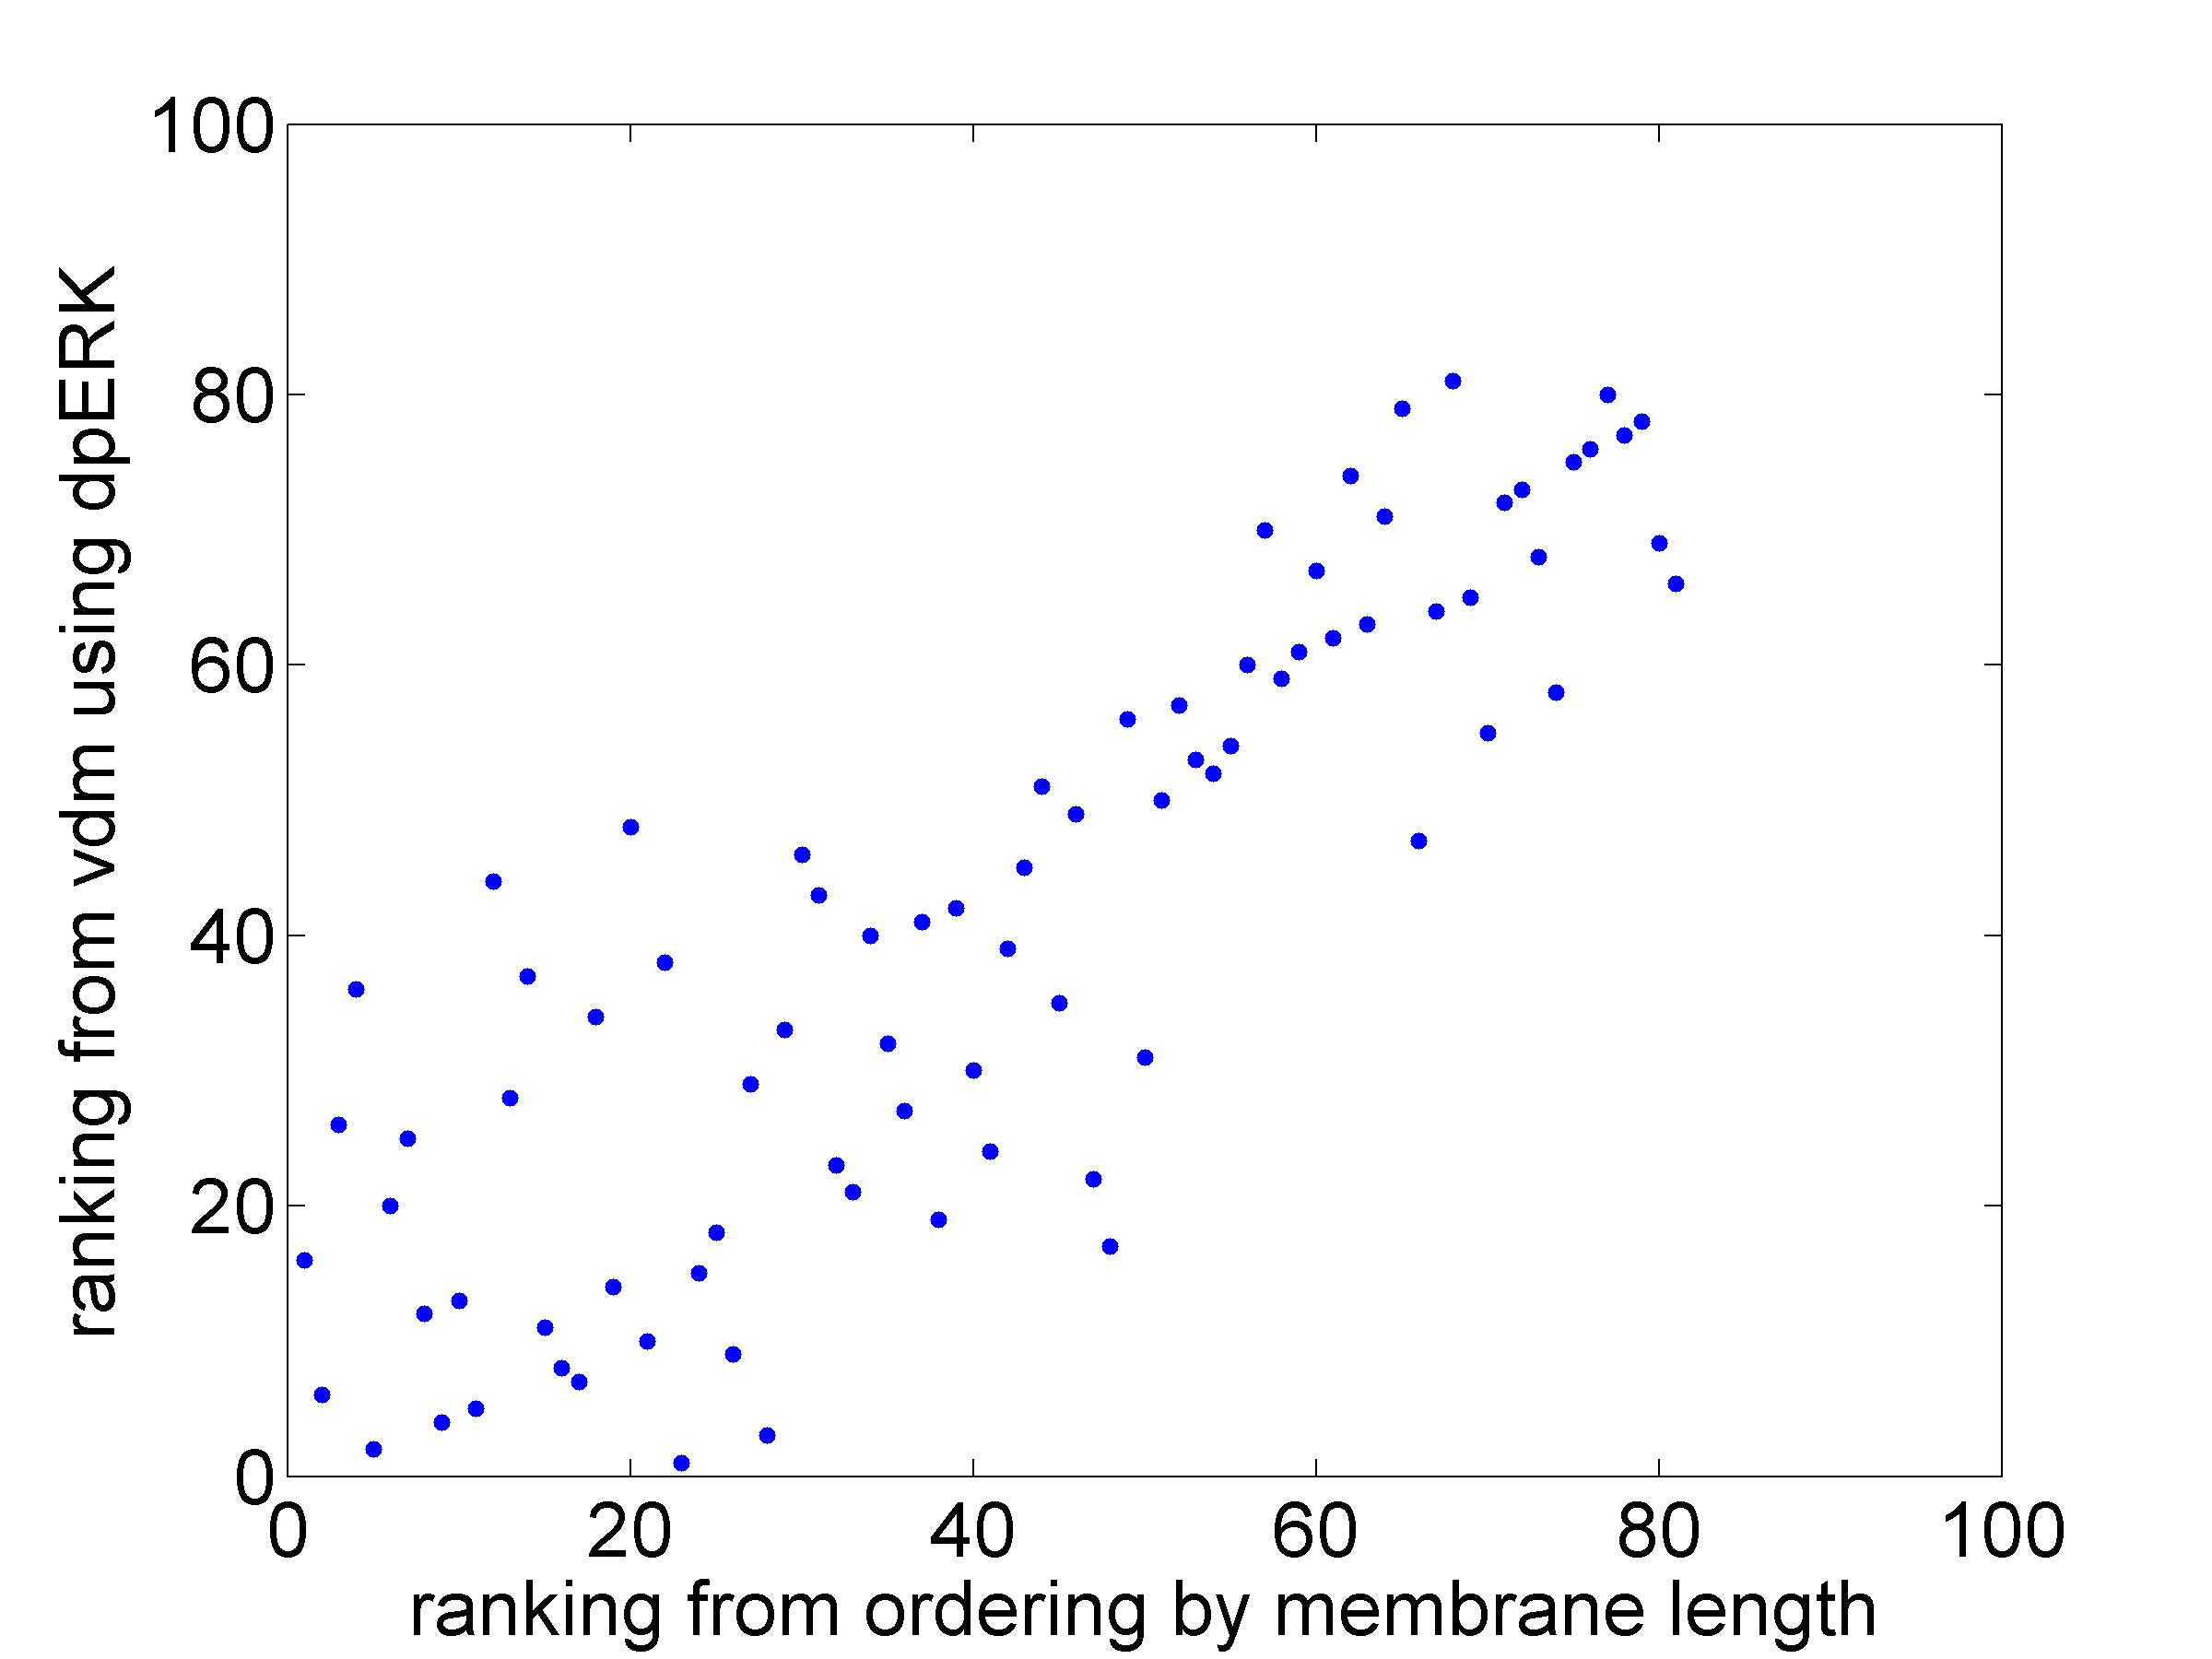
\includegraphics[width=0.45\textwidth]{dpERK_rank_corr}
\end{figure}

\subsection{Dorsal}

\begin{figure}
\begin{minipage}{0.5\textwidth}
\forloop{n}{1}{\value{n} < \nimages}{
	\includegraphics[width=\imagewidth]{DI_\arabic{n}}
	\hfill
}
\end{minipage}
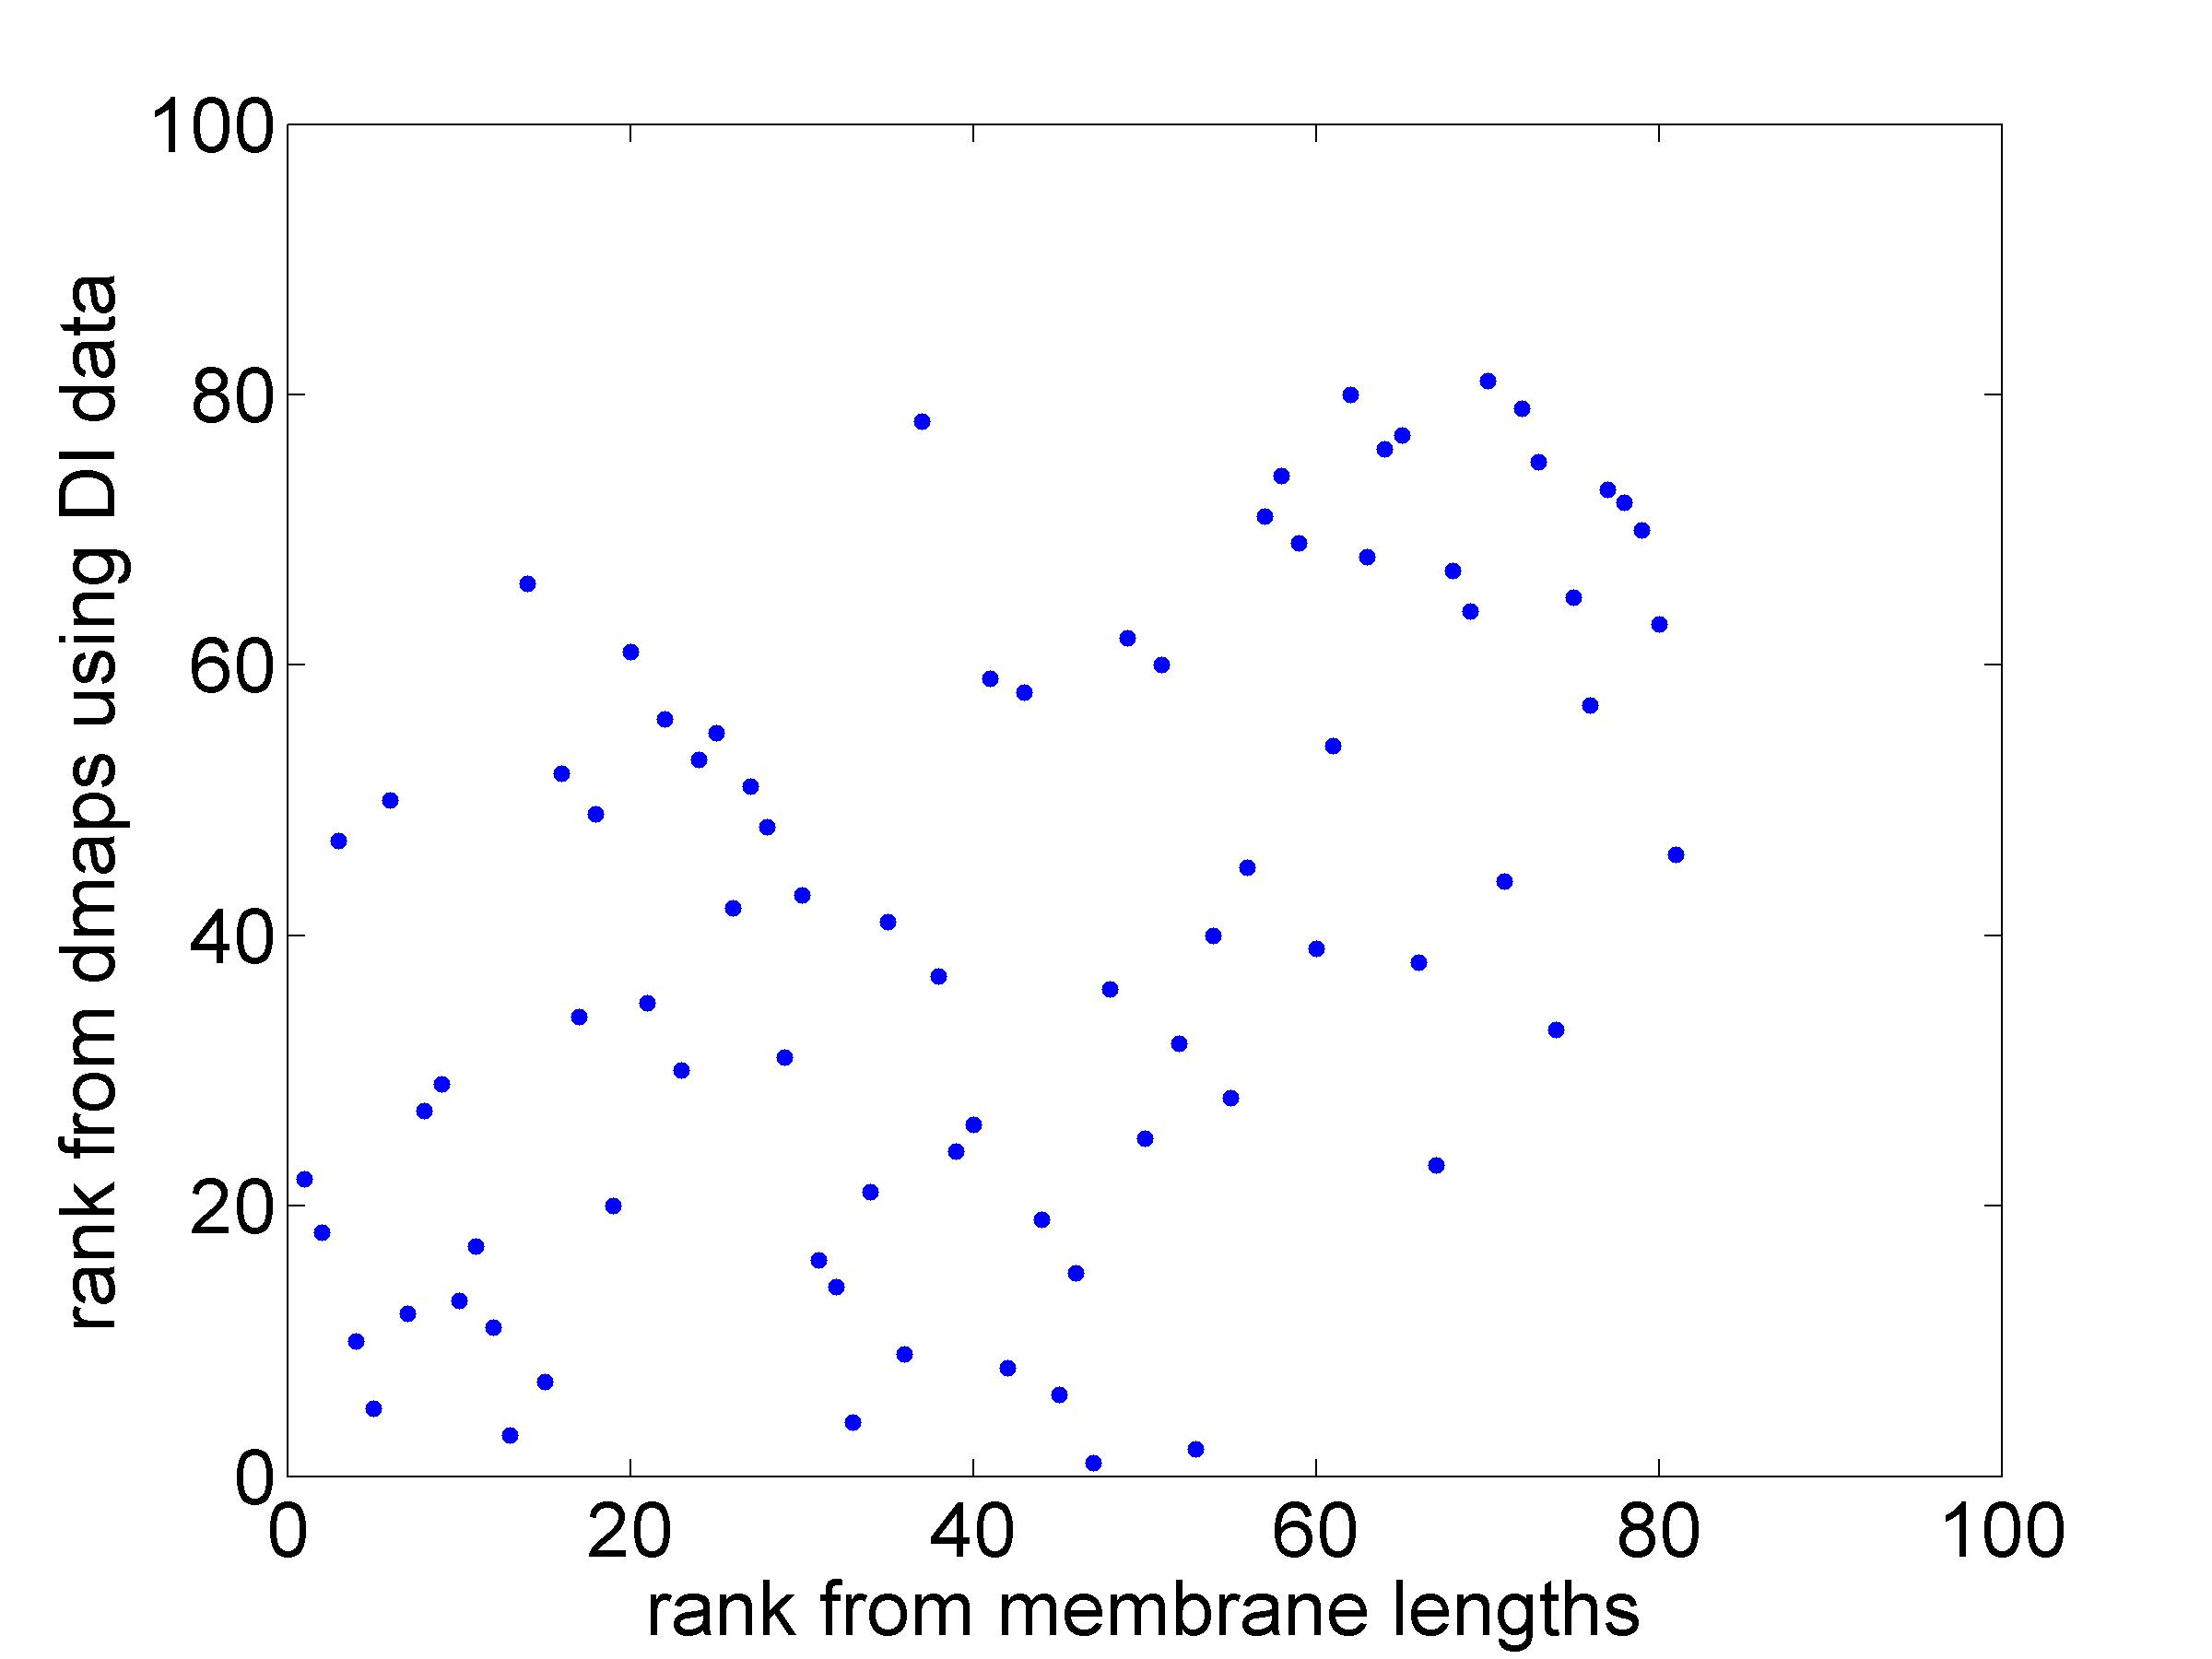
\includegraphics[width=0.45\textwidth]{DI_rank_corr}
\end{figure}

\section{Discussion}
% compare to TSP algorithms

\bibliographystyle{plain}
\bibliography{../../references/references}

\end{document}